%% This document gives an example on how to use the gucmasterthesis
%% LaTeX document class.

%% Use short name MMT MIS or CIMET, and language,  english or norwegian
\documentclass[MACS,english]{gucthesis}

\usepackage[T1]{fontenc}
\usepackage[utf8]{inputenc}     % For utf8 encoded .tex files allows norwegian characters in the files. This can be dangerous if you change to a differnt editor.
\usepackage[pdftex]{graphicx, hyperref}   % For cross references in pdf
\usepackage{color}              % For colouring text   
\usepackage{url}

\begin{document}

\thesistitle{Usable Security Tool for Investigative Journalists}
\thesisauthor{Aneesh Dasari}
\thesissupervisor{Cristina S Marco}
%\thesissupervisorA{Jon Yngve Hardeberg}  % if you have a second supervisor add it like this
\thesisHostInstitution{\GUC}

%\thesisHostInstitution{University of Eastern Finland}

%\thesisjuryA{} %jury names
%\thesisjuryB{} %jury names
%\thesisjuryC{} %jury names
%\thesisjuryD{} %jury names

\gmtkeywords{Thesis, Latex, Template, IMT}
\gmtdesc{This is the short description of a masters thesis}


\thesisdate{\gucthesisdate}
\useyear{2012}


 % this is the file which contains all the details about your thesis
\makefrontpages % make the frontpages

\thesistitlepage % make the ordinary titlepage
\chapter*{Abstract}

Investigative Journalists have been playing a pivotal role in unearthing lot of hidden truths buried under the carpets. They have been instrumental in exposing incompetence, corruption, lies, abuse of power and broken promises etc. In the process of communicating with sources and collecting, analyzing, investigation, disseminating of information, the Interactive tools play a role of catalyst in performance of their job. J.D.Tygar and A Whitten most renowned researchers have identified a “weakest link property". The property states that  stating that muckrakers can exploit when users make error while using the digital tools. 

Therefore a single error made by investigative journalists while using digital tools may lead to loose data and there will be a chance for muckrakers to find out their sources identity. This research is oriented towards the study, evaluation and improving usability of security tools by considering mental model of the investigative journalists. There are many digital security tools currently available for investigative journalists like Tor browser, Text Secure, Red Text and so on for protecting their data and sources. But the tools mentioned above faces usability issues by which users may tend to stop using the tool gradually or may tend to make errors. Most of the security tools available in the market are developed for larger audience and not specifically for investigative journalists and according to Pew research centre many investigative journalists don’t use digital security tools to protect their digital privacy because there more chance for loosing the data and they can be traced by geo-location and so on.

Therefore, in this thesis I will design an application by considering the investigative journalist requirements. Furthermore, the tool will be designed in such a way that both investigative journalists who are technically sound and those are who aren’t; are comfortable in operating/using is also emphasised. Improvisation of usability tools and enabling all the Investigative Journalists to enjoy the fruits of technological breakthroughs, emerging out of day-to-day research work by consolidation and orientation towards employing cognitive walkthroughs, interviews, usability testing.


%\include{summary}

\chapter*{Preface}

I would like to thank Cristina




\tableofcontents

% Comment with a percent to remove figures or tables:
\listoffigures
\listoftables


\chapter{Introduction}
\label{chap:introduction}

It is broadly acknwoledged that security tools are only effective when they are used by all the end users, who are technically savvy and those who aren't. Technically well implemented code will not provide security if users are unable to use the primary features of the tool. Human errors are one of the main reason for most of the security system failures. However, still the user interfaces or the features of the security tool are designed to be clumsy and confusing. Therefore, this research will focus on the need to improve the usability for security tools which are used by investigative journalists like Tor, Cryptocat, TextSecure and so on ~\cite{wm4}. The reasons for the security system failures are assessed by evaluating the existing tools.
\section{Keywords}
Privacy, anonymity, investigative journalist, usability. 

\section{Problem description}\label{Problem:description}
"There is a usability gap that is transformed directly into usage gap", if users don't know how to use the security tool even with appropriate awareness~\cite{furnell2006challenges}. However, this gap may force the end user to stop using the tool or to mis-use the key security features like encryption, public keys, private keys, signatures and so on. Generally, security tools provide privacy and anonymity for the end-users and also protects information from their adversaries. Moreover, privacy and anonymity depends on the set of users using the tools. Larger the set, higher the anonymity and privacy are achieved~\cite{dingledine2006anonymity}. For suppose if the number of users stops using the security tool which provides anonymity and privacy, then privacy levels get decreased for the existing user.  In order to increase  privacy and anonymity levels for both  existing user and new user. The tool should be designed in a way that it can be used by users, who are technologically savvy and also by those who are not. Then, there may be a chance for more numbers users to use the security tool~\cite{pfitzmann2001anonymity}. Therefore, usability affects the security in systems that aim to protect data confidentiality. But when the goal is privacy, it becomes even more important ~\cite{dingledine2006anonymity}.

There are some secured tools like Tor Browser, RedPhone, TextSecure, Cryptocat and so on, which are highly recommended for investigative journalists to protect the data and identity of the sources~\cite{wm4}. Tor browser avoids someone viewing your web history and provides access to sites that are blocked \footnote{https://www.torproject.org}. RedPhone and TextSecure has the capability to secure the exchange of conversations made from their personal mobile phone/smart phones and provide end to end encryption. Chat and Text messages are safe and cannot be decoded even if the phone is lost \footnote{https://whispersystems.org}. Cryptocat provides encrypted chat in browser and mobile phone\footnote{https://crypto.cat}. These tools are technically well implemented, but they are haunted by usability issues like a frequent crash of web pages, missing translations and extraction issues for Tor browser~\cite{pa3}. Connectivity issue within the interfaces due to various configuration for different devices and issues like no feedback to the user is provided when the problem is raised for RedPhone~\cite{sr4}. Duplication of contacts in the contact list and some issues with the color interface design  and feedback to the user for TextSecure~\cite{ti4}. Usability issues due to language differences and lack of cultural integration for Cryptocat~\cite{kobeissi2013cryptocat}.

Investigative journalists spend months or years to verify in-depth truths, discover hidden secrets, shed a spotlight on social justice and accountability, that may involve crime, corruption and corporate wrongdoing etc. During investigating or researching on any social issue, international or any other issues, investigative journalists contact their source and colleagues, located across the globe.~\cite{Ijnet14} They are highly protective about their data and  contacts because adversaries may try to mislead the investigations or threaten investigative journalists; their colleagues and sources. The usability issues that are described above may prevent the investigative journalists to use the features that are essential. These issues may also lead to misuse of features with out the knowledge of investigative journalists. Which results in creating a risk for them, their sources, data and colleagues. At present, It is broadly acknowledged that security requirements can't be addressed by technical means alone, and the chances of success will be essentially affected by the users involved ~\cite{furnell2006challenges}. Therefore, this research will coherently evaluate current existing tools that are used by investigative journalists, explore the challenges of usable security, prevailing problems and propose a usable interactive solution based on observations. 
\section{Justification, motivation and benefits}
The assessment and improvement of security tools in terms of usability are  important for investigative journalists to maintain high privacy and anonymity levels. But if improved, it  helps in minimize the human and interface errors that would occur while using the security tools~\cite{furnell2006challenges}. Chances of risk get decearsed and provides support for investigative journalists to discover hidden truths and perform investigations with regard to social justice.

Many of the previous works have expressed and showed how important it is to improve usability in secure system tools, like in the work done by J.D.Tygar et al ~\cite{whitten1999johnny}. Evaluating the security tool PGP 5.0 to know whether is it usable and produce effective security of most computer users. After evaluating the PGP 5.0 tool, they have observed that   desipte of it's attractive computer interface, it is not usable for most its computer users~\cite{whitten1999johnny}.

The identified problem when solved can be very beneficial for investigative journalists during situations like discovery of truths about government officials (who otherwise are powerful people and any slackness in maintaining secrecy at investigation stage will be hazardous and  may obliterate the whole exercise), investigating about a bank robbery or about any issue when they are accountable for public etc. The soluble will help the investigative journalists to maintain confidentiality of the information and identity of the source from their adversaries.


\section{Research questions}\label{research:questions}
The research questions included in this work are:
\begin{enumerate}
	
	\item How are the existing secured tools used by investigative journalists are user friendly?
	\item How does the existing tools provide a dependable amount of privacy and anonymity while maintaining usability?
	\item If privacy and anonymity are comprised due to design flaws in terms of usability, then how can it be fixed?
	
	
\end{enumerate}

\section{Planned contributions}
In this research the problem addressed above can be solved by considering the previous best resulted works~\cite{whitten1999johnny}~\cite{clark2007usability}. In this work a more structured and precise steps will be implemented by considering most useful factors to find a better solution to the problem. The work from ~\cite{whitten1999johnny}~\cite{clark2007usability}~\cite{furnell2006challenges}~\cite{dingledine2006anonymity}~\cite{kobeissi2013cryptocat}~\cite{katsabas2005using} are extracted and organized to formulate a new methodology to provide a more improved solution to the problem addressed.

 
\chapter{Usability}
 

 
\begin{center}
	
``\textit{The extent to which a product can be used by specified users to achieve specified goals with effectiveness, efficiency, and satisfaction in a specified context of use}” -The definition of usability according to ISO 9241 standard
\end{center}


 \chapter{Literature Review}
 \label{chap:relatedwork}
 First section will give an overview of previous related works  and
 the major contributions regarding usable security are described in this section. Second section illustrates Human computer interaction- security guidelines and  third section describes readical shift and impact of technology on investigative journalists.
 \section{Usable Security}
 
 The concept of usable security was first instigated in 1975 by Saltzer and Schroder~\cite{sasse2005usable}. In their work they have derived design principles for protection of information in security systems and identified the need of physchological acceptability in system that do security operations. The psychological acceptability is defined as ``It is essential that the human interface be designed for ease of use, so that users routinely and automatically apply the protection mechanisms correctly. Also, to the extent that the user's mental image of his protection goals matches the mechanisms he must use, mistakes will be minimized. If he must translate his image of his protection needs into a radically different specification language, he will make errors~\cite{saltzer1975protection}". This statement provides a platform for programmers to design the interfaces by considering the user mental model. Mental model is A mental model is the ``representation that a person has in his mind about the object he is interacting with"~\cite{weinschenk2011100}. \\
 
 The work of J.D.Tygar and A Whitten~\cite{whitten1999johnny}  has influenced most of the programmers and researchers to consider user requirements while designing the security mechanisms and their paper ``Why Jhonny can't encrypt" is widely cited in most of the research works~\cite{clark2007usability}~\cite{dingledine2006anonymity}~\cite{furnell2006challenges}~\cite{katsabas2005using}~\cite{brodie2005usable}. Sometimes the errors made by the users may lead to security failures therefore J.D.Tygar and A Whitten have argued that effective security requires a different usability standard and that is not achieved by using user interface techniques that are applied for designing other softwares. They have defined usability for security as "Security software is usable if the people who are expected to use it:"
  \begin{enumerate}
  	\item are reliably made aware of the security taks they need to perform;
  	\item are able to figure out how to successfully perform those tasks;
  	\item don't make dangerous errors;
  	\item are sufficiently comfortable with the interface to continue using it. ~\cite{whitten1999johnny}
  \end{enumerate} 
  They have also identified five problematic properties of security for user interface design:
  \begin{enumerate}
  	\item \textbf{The unmotivated user property}: The general tendency of the people who use computers is that the information is secured till such time the area of work and use of computer is kept secluded.  Most of the users feel that the information is always secured and are busy in sending emails, download software’s and browse web pages.  Many users are not concerned of the security measures and are of the apprehension that everything is secured and risk free since they have secluded the working area and therefore only concentrate on their work devoid of security measures.  Therefore, the designers of Interface Security cannot be under the impression that the user will go through manuals and look for the security tools that are designed to be self-effacing.  It is also evident that application of security measures in case found cumbersome or unfriendly there is always a tendency of the users avoiding and in search of alternatives.
  	
	\item \textbf{The abstraction property}: Grant of accesses to resources depends on security policies which are systematic and based on abstract rules which are the main criteria to provide accessibility rights.  Programmers while designing such rules makes them as a general task and the same may not be in the knowledge of the general user population.  Therefore, while making the User Interface design for security the programmers need keep this in mind.
	
    \item \textbf{The lack of feedback property}: The system of feedback helps in improvisation of the software and also prevents the possibility of most rectifiable errors and some time prevents serious errors.  However, providing feedback by the users for security management is complex and varies from user to user.  The requirements of the user mainly caters by the correct security configuration and only the user will be aware of the requirements, therefore it is difficult for the software to perform the check of errors.
    
    \item \textbf{The barn door property}:  Even by mistake any time even for a short duration a secret is left insecure there is no guarantee that the same has not fallen into the hands of the attacker.  Therefore, to avoid such incidents the user interface design for security  needs to accord top priority in ensuring that the user is made aware and avoid is making such security mistakes may be sometimes they are too costly.
    
    \item \textbf{The weakest link property}: Even the minutest mistake by the user may give the advantage to the cracker and may be some times end the game.  Therefore, the use needs to be made aware of the security in all aspects.
     ~\cite{whitten1999johnny}
  	\end{enumerate}
  
  To test the hypothesis mentioned above, they have looked for existing software that has good user interface design for security. Therefore they have selected PGP 5.0 for Macintosh as its user interface has appeared to be resonably well designed by general consumer standards~\cite{whitten1999johnny}. They have set minimum usability standard that PGP 5.0 need to meet to enable people to successfully use it to secure their mail.  They have selected two methods to evaluate security tool PGP 5.0: informal cognitive walk-through and usability testing. Cognitive walk-through is a usability evaluation method where a series of tasks and set of question are asked from the perspective of user~\cite[p.84]{baecker2014readings}  and it mainly tends to focus the learnability of the user interface for the users who are technically savvy and for those who are not~\cite{whitten1999johnny}. They have evaluated the visual metaphors, encryption key types, key management policy, key server and irreversible actions of PGP 5.0 tool. As the results drawn from cognitive walk-through mostly rely on the evaluators~\cite[p.84]{baecker2014readings}. To get best results the evaluators should have better knowledge about the user interfaces, therefore J.D.Tygar and A Whitten had conducted usability test to achieve better results. Usability testing is conducted by performing experimental tasks with real users and it helps in finding usability problems before writing any code. Therefore they have designed the test to check whether the PGP 5.0 meets the required usability standards. J.D.Tygar and A Whitten have given a scenario to the participants to do security tasks. After performing both the evaluation methods, they have noted usability problems in PGP 5.0 tool. But the tool is well acknowledged for its design as their marketing literature has stated that `` It has improved graphical user interface makes complex mathematical cryptography accessible for novice computer users."~\cite{whitten1999johnny} \\
  
 Jeremy clark et al.~\cite{clark2007usability}have worked on a privacy tool Tor, that provides anonymous web browsing capabilities. They have evaluated four competiting methods of deploying Tor clients, and number of software tools that have intergrated Tor: vidalia, Privoxy, Torbutton, FoxyProxy and TorPark. They have used cognitive walk-through, which is suggested by J.D Tygar et al to evaluate the tools. They have also considered the usability standard guidelines proposed by J.D.Tygar et al~\cite{whitten1999johnny}. Their aim behind using the cognitive walk through is that users learn by exploring the software interface rather reading the software or user manuals. Due to time and cost constraints they have not performed any usability tests. For conducting cognitive walk-through they have designed core tasks and evaluator will do these taks and evaluate the usability of the application against set of evaluation guidelines which are drawn from ~\cite{chiasson2006usability}~\cite{whitten1999johnny}~\cite{karat2005usability}~\cite{reagle1999platform}~\cite{wharton1994cognitive}, the guidelines used are mainly intended for Tor specifically and the guidelines are:~\cite{clark2007usability}
 \begin{enumerate}
 	\item Users should be aware of the steps they have to perform to complete a core task.
 	\item Users should be able to determine how to perform these steps.
 	\item Users should know when they have successfully completed a core task.
 	\item Users should be able to recognize, diagnose, and recover from non-critical errors.
 	\item Users should not make dangerous errors from which they cannot recover.
 	\item Users should be comfortable with the terminology used in any interface dialogues or documentation.
 	\item Users should be sufficiently comfortable with the interface to continue using it.
 	\item Users should be aware of the application's status at all times.~\cite{clark2007usability}
 \end{enumerate}
 In the work, Challenges of understanding and using security: A survey of end users, S.M.Furnell et al~\cite{furnell2006challenges} had scrutinize the possible usability challenges in security features of end-user softwares. They mainly considered software packages like Windows XP, Internet Explorer, Word and Outlook Express. They have outlined key points that will influence overall usability of the resulting protection~\cite{furnell2006challenges}.
 \begin{enumerate}
 	\item \textbf{Understandable} – Options and descriptions should be presented in a manner that is meaningful to the intended user population. Security offers a great deal of potential for the use of technical terminology and other jargon, but this could easily come at the cost of excluding a proportion of the users. Sufficient help and support should be available to assist novices to achieve the level of security that they need.
 	\item \textbf{Locatable} – Users need to be able to find the features they need. If casual users have to spend too long looking for security, it increases the chances that they will give up and remain unprotected.
 	\item \textbf{Visible} – The system should give a clear indication of whether security is being applied. Appropriate use of status indicators and warnings will help to remind users in cases where they may have forgotten to enable appropriate safeguards.
 	\item \textbf{Convenient} – Although visibility is important, the provision of security should not become so prominent that it is considered inconvenient or intrusive. Users are likely to disable features that become too much of an impediment to legitimate use.~\cite{furnell2006challenges}
 \end{enumerate}
 They have conducted a survey to assess end-user understanding of security features in common software applications. The researchers~\cite{furnell2006challenges} have felt that respondents would feel more comfortable and interested in answering the questions about programs they were familiar with. Therefore they have selected above tools as they are well known and widely used. They haven't use cognitive walk through or the usability test because survey findings offer a revealing insight into difficulties that may lay users are likely to experience when attempting to understand and use the security aspects of the software placed before them. Total of 342 responses are recorded during the survey period. The questionnaire began by asking whether the users are aware of security feautures in software packages mentioned above. The survey findings have identified that most of the users could not able to understand  or dont know the security features of the mentioned packages. For example in regard to the security features related to Microsoft outlook express the findings revealed that 65 percent of the respondents did not understand the meaning of digital ID and 61 percent of the respondents did not understand the use of term encrypt. Based on the findings of survey conducted on widely used software packages portray that security features should be designed in a way that most of its users should understand in using it. S.M.Furnell et al~\cite{furnell2006challenges} has suggested that default settings of the security features of an application should provide sufficient protection for majority of users using the application ~\cite{furnell2006challenges}. 
 
 \section{Guidelines}
 Katsabas.D, et al.~\cite{katsabas2005using} in their work used number of Human computer interaction applied in area of security and had evaluated three anti-virus applications: Norton Antivirus, Panda Antivirus,Agnitums Outpost Firewall, Zone Alarm Firewall, McAfee Virus Scan, as well as Opera and Mozilla Firefox web browsers, Qualcomm's Eudora, Incredimail email client software and finally Microsoft Word. These applications are evaluated by conducting usability test and evaluated according to the level of attention that they afforded to have key issues. The software tool Mozilla Firefox obtained relatively low score, as it did not satisfy most of Human computer interaction guidelines that applied in security area. Most of the guidelines are drawn from Johnston et al~\cite{johnston2003security} work and other guidelines are created by modifying 10 usability heuristics proposed by Nielsen. They have proposed ten guidelines  and the applications mentioned above are evaluated against each one of them.~\cite{katsabas2005using}
 \begin{enumerate}
 	
 	\item \textbf{Visible system state and security functions}: The users are not expected to search for security tools or find hidden security tools hidden inside the application.  The users are always kept aware and informed about the state of system by the use of status mechanisms and therefore the status information should be automatically updated and easily accessible.
 	
 	\item \textbf{Security should be easily used}: The security settings should not be scattered at different places and interface should be so designed that the user may utilize the security features with less effort and easily accessible. 
 	
 	\item \textbf{Suitable for advanced as well as first time users}. The application of security should be designed in such a manner that even the first timer can use it easily and the information so provided should not be lengthy that the advanced user also can refresh.  To better the usage of software more easily and quickly shortcuts may be provided.
 	
 	
 	\item \textbf{Avoid heavy use of technical vocabulary or advanced terms}: It is always better to use simple language and avoid technical vocabulary and advanced terms so that it is easy for the beginners to apply the security features. 
 	
 	\item \textbf{Handle errors appropriately}:Application needs to be planned cautiously in such a manner that errors which occur while making use of security measures can be prevented or minimized as much as possible.  Pop ups of error messages should be evocative and problem solving.
 	
 	
 	\item \textbf{Allow customization without risk to be trapped}: Default values should be easily and automatically restored by providing exit paths when by mistake some wrong functions are chosen.
 	
 	
 	\item \textbf{Easy to setup security settings}: Enabling easy to setup security settings will make the user more confident and help in changing and configuring the application need based.
 	
 	
 	\item \textbf{Suitable Help and documentation for the available security}: To assist the users when they face difficulties, suitable help and documentation should be provided to ease out and overcome the problems.
 	
 	
 	\item \textbf{Make the user feel protected}: The application needs to assure the users that their work is totally protected.  Application should make sure that the users do lose the data when unexpected errors are made and the recovery of data is easy without any loss.  Latest security features should be incorporated so that the user feels highly protected. 
 	
 	\item \textbf{Security should not reduce performance}: Application of security features should be so designed by applying efficient algorithms so that there is smallest amount of impact on the effectiveness of the application.~\cite{katsabas2005using}	
 	
 \end{enumerate}
 \section{Technological impact on investigative journalists}
 In this section the problems faced by investigative journalists due to technology are discussed as it's already said in the above section that it is important to know the mental model of investigative journalists for minimizing the rate of occurence of errors.	Firstly, the technological changes are being discussed and followed by the postives of technological shift are discussed. Then problems arised due to radical change in technology are discussed.\\

 Investigative reporting was developed during the 18th century, mainly in France, England and American colonies. In the early years of 19th century it was admired by public for its accountability and social justice and by the end of world war II the traditional approaches/techniques like interviews, tracking public documents and so on are well understood by the practioners.~\cite{defleur2013computer} During 1980's, world with the emergence of high-speed technology like internet~\cite{kawamoto2003digital}, personal computer, video cassette recorder~\cite{5oxford2009} and so on,  changed the traditional journalism into digital journalism with the emergence of new tools and practices that are redefining the place of journalism. This change is called as Journalism 2.0 by researchers and journalists ~\cite{kaul2013journalism}. The fusion of computer power and news reporting sometimes called computational journalism''~\cite{flew2012promise}. According to Hamilton and Turner (2009)~\cite{hamilton2009accountability} computational journalism supplement the accountability functions of journalism by bringing algorithms, data and social science together. Diakopoulos et al. (2010)~\cite{diakopoulos2010diamonds} suggest that computational journalism helps journalists in doing their work, such as by providing visualization tools and filtering source information. According to Lewis and Usher (2013)~\cite{lewis2013open} many scholars argued that computational journalism will lead to better investigative journalism and new forms of engagement are created with end-users or audience.\\
 
 (Steensen (2011)~\cite{steensen2011online}, in their research work have measured the success rate of online journalism based on interactivity, multimedia and hypertext and these are called as technological assets. Hypertextuality is about linking and layering of digital information through  a hierarchial structure. interactivity is all about engaging user participation in the process of information seeking and sharing and the use of more than one type of media in a single device or product ~\cite{steensen2011online}. They have also stated that these technological assets have a greater impact on online journalism, which is also called as digital journalism. Kawamoto (2003)~\cite{kawamoto2003digital} has defined digital journalism as ``The use of digital technologies to research, produce, and deliver news and information to an increasingly computer-literature audience." ~\cite{kawamoto2003digital} have drafted the characteristics that are typical online journalism: Hypertext, customization, convergence, personalization and nonlinearity to the technological assets. They have also stated in their work that if there is a change in technology then the concept of journalism changes and the definition of digital journalism also changes.\\
 
 The technological advancements/breakthroughs like internet, email service, voice and video chat etc., helps the reporters to have direct contacts with their editors and contacts all over the globe. The greater use of data analysis, web software by journalists, computer scientists and citizens has incommensurate increased in the recent past. In this advanced environment where the journalists at present work, new realities are uncovered every day, audience feedback is integrated; more differing viewpoints on the same stories are consistently introduced; more stories are accessible and searchable~\cite{van2012future}. Mosco (2004) ~\cite{mosco2004digital} argues that ``the entry of new technologies has always been surrounded by Myths about their revolutionary power" like an iPod which made stronger impact on the growth of technologies. Entry of new technologies have always been revolutionary, create enormous power and surrounded by myths about their capabilities.  The rise of machines (computers and their software) and networks have played major role in creating future for investigative journalism.\\
 
 These factors mean more focus to the investigative journalism itself, more citizen involvement in shaping stories, and more collaboration. As Knight foundation encourages~\cite{3media2014} - investigative journalism itself focus on involvement of more citizens in shaping stories resulting in more collaboration than competition. In fact, the past few years have seen remarkable growth in non-profit newsrooms and greater use of data analysis and Web software by groups composed of journalists, computer scientists, and citizens. These initiatives then use new technology to create networks of newsrooms to share information, to improve the quality of their investigations, and to create cost efficiencies. It is no exaggeration to state that the new technologies have transformed the practices of investigative journalists all over the world and Norway has not been an exception. ``As Norway was among the first countries to connect to the internet and according to the Jupiter research, Norway is one of the most digitally advanced markets in Europe" ~\cite{ottosen2012digital}. The impact of new technologies on investigative journalism has revealed dialectical impact and suggests that the Internet, email and cellular phone play a pivotal role in enhancing the results in reporting.  These gadgets have strengthened the Journalists in meeting their day-to-day requirements of collection, investigation and interaction which are the main elements in cracking the stories and bringing the truth out.\\
 
 Alan Rusbridger has stated that ``All journalism is investigative to a greater or lesser extent, but investigative journalism it is a bit of a tautology is that because it requires more, it's where the investigative element is more pronounced." ~\cite[p.17]{de2008investigative}  Therefore, the effect of technology on journalism also implies to the investigative journalism. According to Franco (2009)~\cite{gf9} the impact of digital technology on journalism occur in three principal categories.
 \begin{enumerate}
 	
 	\item The dynamics of news and information generation
 	
 	\item Professional practices and skills that are necessary in digitized environment
 	
 	\item Situation of traditional media.
 	
 \end{enumerate}

 There are several databases like Government websites, News organization databases and other nonprofit organization databases  (Hate speech International Norway, Icelandic Centre for Investigative Journalism Iceland, the Norwegian Foundation for Investigative Journalism (SKUP)) available for investigative reporters to get access to or to retrieve the documents that are important for journalists to do in-depth research.~\cite{knight2001online}. Computer Assisted reporting helps the journalists to store the procured data into a software like google spreadsheets, Microsoft excel sheets or other statistical packages for analysing the information. Both databases and Computer assisted reporting provides an overview of the story, which is being researched by the journalist. There are a number of methods and tools already available for retrieving the documents from the massive database for journalists, some of them are google fusion tables, google public data explorer, google refine etc.~\cite{defleur2013computer}\\
 
 Ottosen and Krumsvik (2012)~\cite{ottosen2012digital}, in their research work, have reflected the survey conducted by Norwegian union of journalists in 2007 among 715\footnote{Sample includes all members of the
 Norwegian Union of Journalists working on digital and multimedia platforms} journalists in digital media. The findings show that majority of the journalists who have participated in the survey believed that digitization of the work environment help in maintaining positive relationships with their colleagues, improves the relationship with management and they felt comfortable when the digital platform is introduced but some of them claimed that they are worse off than before. The participants also suggested some valuable suggestions for a better journalism. The suggestions include, better conditions for investigative reporting, opportunity to specialize and to do more in-depth work in their own stories, more discussions in the newsrooms. But in a survey conducted by Pew research center~\cite{ia2p}  fifty percent of investigative journalists said that their organizations are not providing enough resources to protect their identity, data and sources from adversaries. Fourty seven percent of them said that their respective organization are providing valuable digital protection resources. In this survey, 671 investigative journalists consisted editors, producers, photo journalists etc, responded to online survey. All the respondents of survey are members of Investigative Reporters and Editors, Inc. (IRE)~\cite{ia2p}. \\
\begin{figure}[ht!]
	\centering
	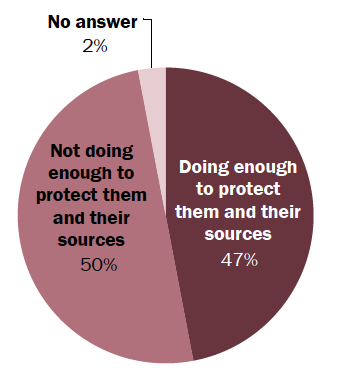
\includegraphics[width=60mm]{1.png}
	\caption{Investigative journalists respond on resources provided by their orgnizations, Pew research center ~\cite{ia2p}.}
	\label{fig:0}
\end{figure} 

 The internet has become a new tool or source for investigative journalists~\cite{knight2001online}. Internet offers accessible sources for journalists to research or investigate. Some of them are Non-government organizations, official government sources, Databases, Computer Assisted Reporting (CAR) etc, the one thing that the journalists resources can do for reporters to make reporting easier. Presently, most of the governments all over the world have gone online. The policy documents, responsibilities, data, press release, materials, etc. related to government institutions are included in the government official websites. Thus, it is easier for the journalists to search for relevant documents, when required to research on any issue. According to the survey conducted by Pew Research Center~\cite{ia2p}, only two percent of the investigative journalists have a lot of confidence on Internet service providers(ISP's). Seventy one percent of the respondents doesn't have confidence on  Internet service providers(ISP's), shown in figure~\ref{fig:1}. The reason for not depending on ISP's due to digital threats like surveillance and hacking. ~\cite{ia2p} \\
 \begin{figure}[ht!]
 	\centering
 	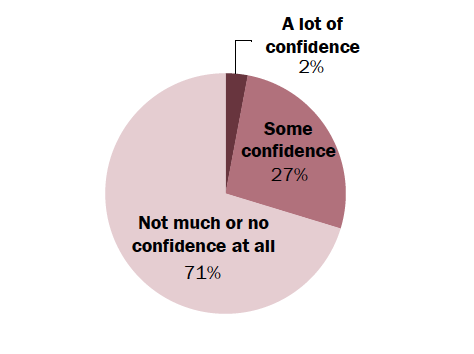
\includegraphics[width=100mm]{2.png}
 	\caption{Level of confidence on Internet Service Providers, Pew research center ~\cite{ia2p}.}
 	\label{fig:1}
 \end{figure}

Most of the news organizations, investigative journalists and other journalists came to know more about surveillance systems when Edward Snowden ~\cite{si4}revealed about the PRISM surveillance system of the United States of America. Most prominent U.S technological companies like Google, Apple, Microsoft etc provide information to Prism system through National security agency(NSA) to keep surveillance on specific people. Journalists comprising of different fileds came to realize that every electronic communication like email, messaging, phone calls and so on are being recorded, stored and analyzed~\cite{si4}. These advances are obtained by government institutions to keep an eye on their public and press. According to the survey conducted by Pew Research Center~\cite{ia2p}, most of the investigative journalists in United states of America feel that their government has already collected their data(phone call or online communication), figure~\ref{fig:2}. Therefore,  Investigative journalists are more worried about protecting the identity of sources and the data (contact information, the story  data, facts and so on)~\cite{wm4}. Investigative journalism is a high risk profession  and some times investigative journalists are targeted even if he/she is not working on sensitive story because their colleagues may work on sensitive stories. Then adversaries may target the respective journalists in order to dig into the issue~\cite{si4}.\\
 \begin{figure}[ht!]
 	\centering
 	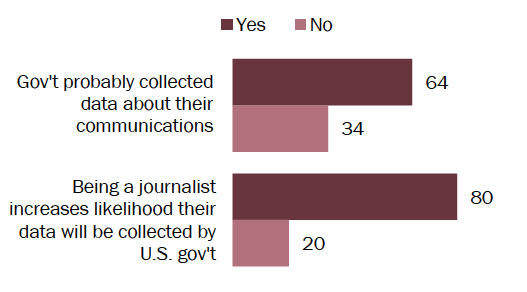
\includegraphics[width=100mm]{3.png}
 	\caption{Data collected by U.S government, Pew research center ~\cite{ia2p}.}
 	\label{fig:2}
 \end{figure}

There are other surveillance systems like Prism  that are operated by some government institutions to track the data. Iran utilizing a surveillance system\footnote{http://news.bbc.co.uk/2/hi/technology/8112550.stm} that is developed by Nokia-Siemans Networks, Libya uses a system developed by Amesys and other companies\footnote{http://online.wsj.com/news/articles/SB10001424053111904199404576538721260166388?mg=reno64-wsj\&url=http\%3A\%2F\%2Fonline.wsj.com\%2Farticle} (French company) , Unite States of America uses a surveillance system called PRISM\footnote{www.theguardian.com/world/2013/jun/23/edward-snowden-nsa-files-timeline} maintained by National Security Agency (NSA). Due to these type of digital threats most of them  have started using digital tools like TextSecure for secure online chat, RedPhone for a secured phone communication, Tor for anonymous web browsing and many.  According to the survey conducted by Pew Research Center~\cite{ia2p}(figure~\ref{fig:3}), 14 percent of respondents revealed that they have stoped contacting their sources due to surviellance systems and three percent of them had stoped covering the senstive stories. Half of the respondents have changed their way of storing/sharing sensitive documents and 38 percent of respondents have changed their way of communication to contact their sources. \\
 \begin{figure}[ht!]
 	\centering
 	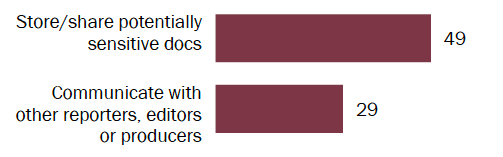
\includegraphics[width=100mm]{4.png}
 	\caption{Changing ways to collet data and to communicate with adversaries, Pew research center ~\cite{ia2p}.}
 	\label{fig:3}
 \end{figure}
Most of the investigative journalists started using secured digital tools to store documents, to communicate with their colleagues or sources. After snowden disclosure about the surviellance system at United States of America(U.S.A), most of the investigative journalists are afraid to rely on digital tools beacuse most of the tools are geo located and adversaries can easily locate them at a faster rate. According to the survey(PEW Research center)~\cite{ia2p} nearlly half of the respondents(figure~\ref{fig:4}) are not using any one of the tools that are classfied in survey. The survey researchers have included tools from email encryption to turning off geolocation on mobile devices~\cite{ia2p}. Description about tools are not revelead in survey because of security issues.\\
 \begin{figure}[ht!]
 	\centering
 	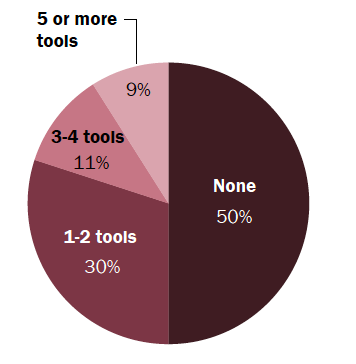
\includegraphics[width=60mm]{5.png}
 	\caption{Use of digital secured tools by investigative journalists according to Pew research center ~\cite{ia2p}.}
 	\label{fig:4}
 \end{figure}
 
 This is my first git hub project 
 
 
 \section{Digital tools}




 
\chapter{Methods}
 Research methods are classified in to two types 1) Qualitative Method and 2)Quantitative Method ~\cite{lazar2010research}. In our research, we are implementing the Qualitative method. To address the first and second research question, we will perform a case study on  three existing tools described in ~\ref{Problem:description}: Cryptocat, TextSecure and RedPhone. The case studies in human computer interaction(HCI) have four goals:~\cite{lazar2010research}
 \begin{enumerate} 
 	\item \textbf{Exploration}: Understanding the problems or situations, often with the hopes of informing new design.
 	\item \textbf{Explanation}: Developing models that can be used to understand a context of technology.
 	\item \textbf{Description}: documenting a system, a context of technology use, or the process that lead to proposed design.
 	\item \textbf{Demonstration}: Showing how a new tool is sucessfully used.~\cite{lazar2010research}
 \end{enumerate}
 Therefore, the case studies helps us in understanding the problems faced by investigatice journalists while using the digital security tools and it will also  help in developing a process based on the results. There are four components of a case study design: research questions; hypothesis or propositions; units of analysis;data analysis plan. Research questions describes the goals of thesis and hypothesis or propositions are the statemetns of what you expect to find. The unit of analysis determines the focus group and finally data analysis plan is helpful in planning the data collection.~\cite{lazar2010research} The research questions are mentioned above in section ~\ref{research:questions}and~\ref{Problem:description}. The unit of analysis is a group of investigative journalists and in this research work the data analysis plan start firstly by  employing cognitive walkthrough method to  evaluate the digital security tools mention in section ~\ref{Problem:description}, as it has been used previously by the researchers mentioned in section~\ref{chap:relatedwork}. Cognitive walkthroughs are often very good at identifying certain classes of problems, especially showing how easy or difficult a system is to learn or explore effectively – how difficult it will be to start using that system without reading the documentation, and how many false moves will be made in the meantime.~\cite{wharton1994cognitive}\\
 
 
 hieeieieieie
 
 In cognitive walkthrough, set of core tasks are developed and these tasks are designated differently for the three digital security tool mention above. We will perform these tasks and evaluate the usability of three security tools: Cryptocat, TextSecure and RedPhone against set of guidelines. These guide lines are to be derived from the previous works~\cite{whitten1999johnny}~\cite{clark2007usability}~\cite{katsabas2005using}~\cite{furnell2006challenges}. To address the third reseach question, although the results from the cognitive walkthrough may provide valuable information regard to the problems faced in existing tools. In this research we will also use contextual inquiry to draw the user requirements. It is one of the best methods to understand the users' work context and it is basically a structured field interviewing method.\\
 
 Contextual inquiry is more a discovery process than an evaluative process; more like learning than testing. This technique is best used in the early stages of development, to gain and understand  how people feel about their jobs; how they carry out their work; how information flows through the organisation, etc.~\cite{1_holtzblatt_2014} According to ~\cite{4nielsen2014} stated that ``The best results come from testing no more than 5 users" because at the best they provide better results. Therefore, contextual inquiry for this research work, we will test no more than 5 users.   Based on the results from cognitive walkthrough and contextual inquiry, we will develope a paper portotype. \\
 
 After developing a paper prototype, we will use the method card sorting,  it helps in understand the investigative journalists expectations. Card sorting is a method The card sorting helps in designing the information architecture according to user needs. By conducting card sorting, there is a chance for getting more insights from the users. 
 ~\cite{2_hudson_2014} Then by considering results that are dervied from card sorting, cognitive walkthroughs and contextual enquiry, we will design the high fidelity prototype. Prototype which is close to the final product. Then perform a usablity testing for evaluating high fidelity prototype, as it produces more objective results. A usability test is conducted to draw the usability problems and this method is conducted mostly in earlier stages or the final stages of the designing process. For conducting the usablity test we will design a real test scenario and ask the users to use the prototype in realtion to scenario.  



\bibliographystyle{gucthesis}
\bibliography{MastersExample}

\appendix
\include{appendix}

\end{document}
